\section{Results}
Our simulator was designed to be similar to the experiments made by Sugiyama
et al.\cite{sugiyama} since data can be compared. Figure (FIXME::) shows
the absolute position on the circular road of all the 60 cars with normal
drivers for $ 150 \unit{s} $. In this plot it can be seen that several of the
cars come to a complete stop after $ 30 \unit{s} $. These stops can then be
characterized as waves \cite{mit} that are moving backwards in the lane with
a constant speed of (FIXME: speed).\\\\


In figures (FIXME: ) there are data from the simulator when the cars are
equipped with ACC and EACC respectively and the jam dynamics can be seen. In
these cases the cars are never forced to stop completely. When the cars
are equipped with ACC the jams does not occur until after $ 300 \unit{s}
$. If they instead are equipped with the enhanced model the jams do not occur
until after $ 1200 \unit{s} $. In both these cases the waves are travelling
backwards in a speed of $ (FIXME:) 18 \unit{km/h} $.



\begin{figure}[h!]
    \begin{center}
    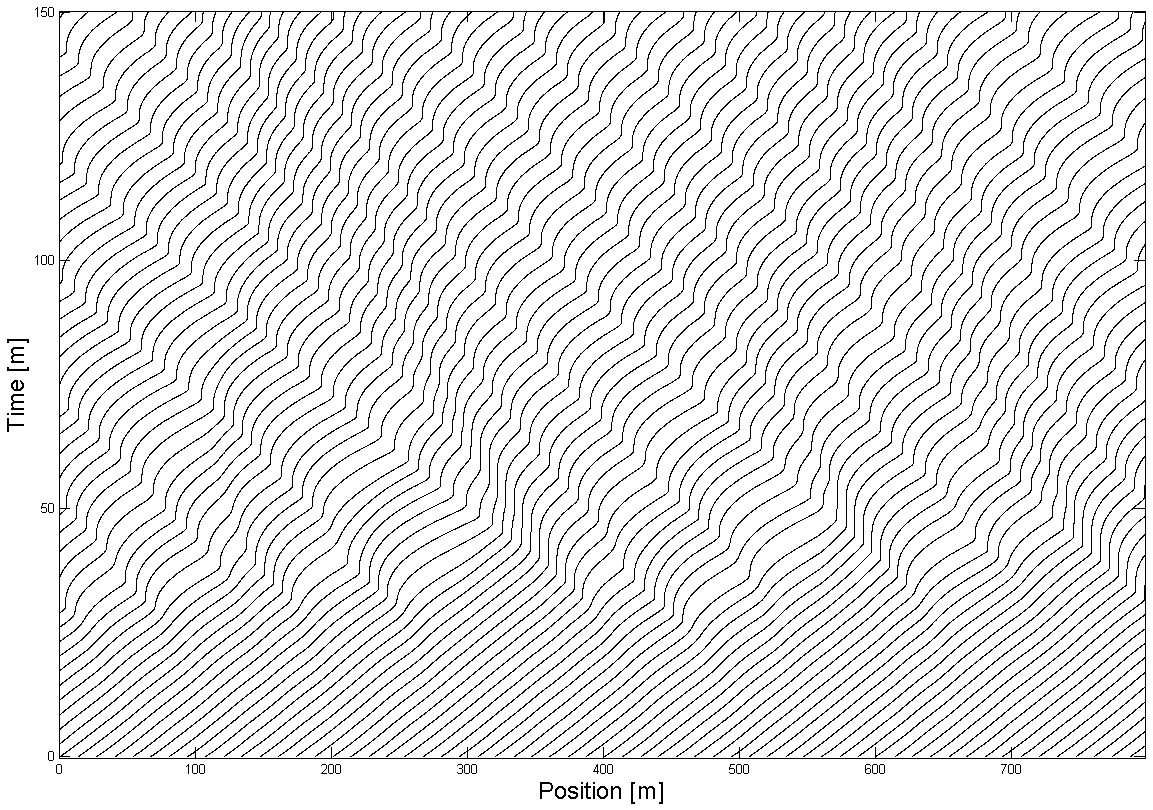
\includegraphics[width=0.8\textwidth]{normal_60cars_50kmh.png}
    \caption{\label{normal_postime}
Absolute position of 60 cars for $ 150 \unit{s} $. Data from simulator. After $ 30 \unit{s} $ phantom jams are emerging.}
    \end{center}
\end{figure}

% Ska vi ha velocityplotten?

\subsection{Comparison of Performance}
We measure performance of the different systems as average traffic flow
$ [\unit{vehicles/h}] $ as a function of average traffic density
$ [\unit{vehicles/km}] $. The speed limit was fixed to $ 50 \unit{km/h} $ in all
experiments. Data is presented in fig \ref{performace}.\\\\

Initially, the performance of all three systems grow linearly as traffic is
light enough to allow all cars to keep maximum allowed speed. As traffic grows
denser, the cars have to slow down to keep constant time headway. All three
system follow the same performance curve until a density of $ 50.0
\unit{vehicles/km} $ is reached. At this point, phantom jams appear in the
\emph{normal driver} system and traffic flow drops dramatically. For the
\emph{Adaptive Cruise Control} system and the \emph{Enhanced Adaptive Cruise
Control} system, phantom jams were first observed at $ 56.3 \unit{vehicles/km} $
and $ 68.8 \unit{vehicles/km} $ respectively. Fig \ref{performance} also shows
that the performance of these two systems is not reduced by the phantom jams
as severely as for the \emph{normal driver}.

\begin{figure}[h!]
    \begin{center}
    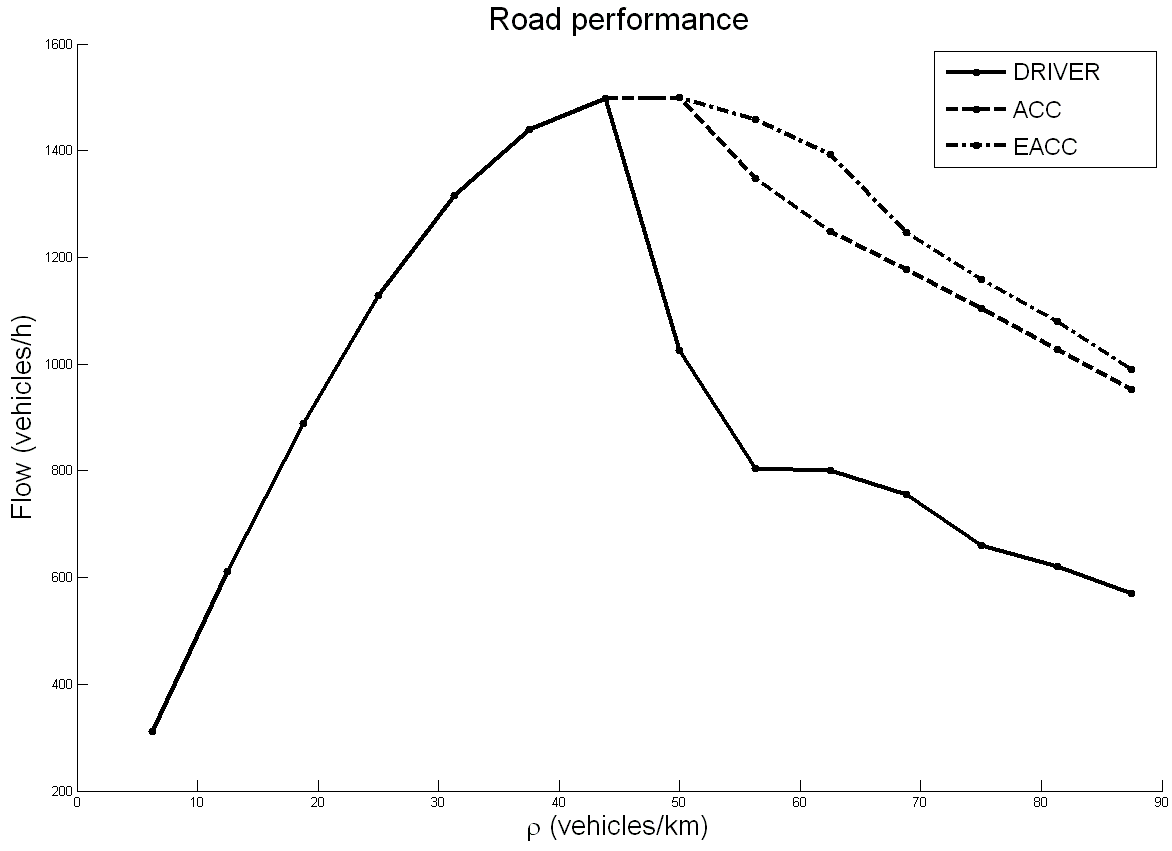
\includegraphics[width=1.0\textwidth]{flowdensity_2.png}
    \caption{\label{performance}
Traffic flow as a function of traffic density. Data from simulator.
$ RoadLength=800 \unit{m} $, $ SpeedLimit=50 \unit{km/h} $, $ TimeHeadway=1.5
\unit{s} $. Traffic flow was measured when traffic conditions had stabilized.}
    \end{center}
\end{figure}


